




% \subsubsection{Framework Overhead}
% \label{sec:framework-overhead}

% A critical first step in evaluating multi-agent orchestration frameworks is to quantify the \emph{baseline overhead} they introduce relative to a direct Large Language Model (LLM) invocation. This experiment isolates orchestration cost from advanced capabilities such as tool use, memory, multi-step reasoning, or inter-agent coordination, and establishes a reference point against which all subsequent results can be interpreted. \textbf{Evaluation Setup:} We evaluate \emph{all supported frameworks} under a unified experimental harness using the same trivial query (\emph{``What is 2+2?''}), the same underlying model (\emph{gpt-4o-mini}), and identical execution conditions. Each framework is configured in its \emph{minimal viable setting}, disabling optional features wherever possible to focus purely on orchestration effects. The comparison includes a raw \emph{Direct LLM} call as a lower-bound baseline; lightweight graph-based and role-based agent runtimes (\emph{LangGraph}, \emph{OpenAgents}, \emph{AutoGen}, \emph{CrewAI}, \emph{Agno}, and the \emph{OpenAI Agents SDK}); and the generative-agent-based modeling (GABM) system \emph{Concordia}. Each configuration is executed for 50 trials under a fixed concurrency level of four, and we report latency, throughput, and output size to capture complementary dimensions of efficiency.




% 


\captionsetup[subfigure]{font=scriptsize}
\begin{figure}[t]
%\centering
\begin{subfigure}{0.57\linewidth}
% %\centering
\begin{tikzpicture}
\begin{groupplot}[
    group style={
        group size=1 by 2,
        vertical sep=0.4cm, % Gap between the two plots
        x descriptions at=edge bottom, % Only show x labels on bottom plot
    },
    width=1.25\linewidth,
    symbolic x coords={LLM,OA,AG,LG,CA,Ag,OS,Co},
    xtick=data,
    ybar,
    % bar width=3pt,
    /pgf/bar width=3pt,
    enlarge x limits=0.15,
    ymajorgrids=true,
    grid style={dashed,gray!30},
    tick label style={font=\tiny},
    ylabel style={font=\tiny},
    xlabel style={font=\tiny},
    every axis plot/.append style={fill opacity=0.9},
    nodes near coords,
    nodes near coords style={
        font=\tiny, yshift=7pt, xshift=5pt, anchor=south, rotate=90
    }
]

% --- TOP PLOT (Outlier Range) ---
\nextgroupplot[
    height=2.5cm,
    ymin=44, ymax=70, % Range for Concordia
    ytick={40, 50, 60},
    axis x line*=top
, % Hide the x-axis for the top part
    legend style={
        at={(0.02,0.98)},
        anchor=north west,
        font=\tiny,
        legend columns=-1
    },
    ylabel={Latency (s)},
    ylabel style={at={(axis description cs:1.03, -1.2)}, anchor=west}, % Centered label
]
\addplot+[fill=blue!60] coordinates {
    (LLM,0.379) (OA,0.495) (AG,0.496) (LG,0.524)
    (CA,0.611) (Ag,0.860) (OS,1.170) (Co,44.473)
};
\addplot+[fill=green!60] coordinates {
    (LLM,0.730) (OA,0.840) (AG,0.787) (LG,1.093)
    (CA,0.801) (Ag,1.183) (OS,2.036) (Co,53.420)
};
\legend{p50, p95}

% --- BOTTOM PLOT (Main Data Range) ---
\nextgroupplot[
    height=2.3cm,
    ymin=0, ymax=3, % Range for all other agents
    ytick={0, 1, 2, 3},
    axis x line*=bottom,
    xticklabel style={rotate=90, anchor=east, font=\tiny},
    % axis y discontinuity=parallel, % Adds the visual "break" symbol
]
\addplot+[fill=blue!60] coordinates {
    (LLM,0.379) (OA,0.495) (AG,0.496) (LG,0.524)
    (CA,0.611) (Ag,0.860) (OS,1.170) (Co,44.473)
};
\addplot+[fill=green!60] coordinates {
    (LLM,0.730) (OA,0.840) (AG,0.787) (LG,1.093)
    (CA,0.801) (Ag,1.183) (OS,2.036) (Co,53.420)
};

\end{groupplot}
\end{tikzpicture}
\vspace{-7mm}
\caption{Latency}
\end{subfigure}
% \hspace{1mm}
% \hfill
% ---------------- Throughput ----------------
\begin{subfigure}{0.42\linewidth}
%\centering
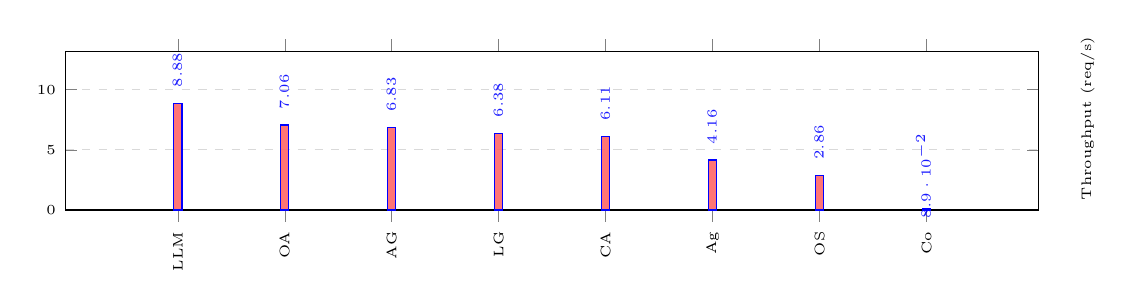
\begin{tikzpicture}
\begin{axis}[
    width=1.15\linewidth,
    height=3.6cm,
    ymin=0,
    ymax=13.206,
    % symbolic x coords={Direct LLM,OpenAgents,AutoGen,LangGraph,CrewAI,Agno,OpenAISDK,Concordia},
    symbolic x coords={ LLM,OA,AG,LG,CA,Ag,OS,Co},
    xtick=data,
    xticklabel style={rotate=90, anchor=east, font=\tiny},
    ylabel={Throughput (req/s)},
    ylabel style={at={(axis description cs:1.05,0.)}, anchor=west},
    tick label style={font=\tiny},
    ylabel style={font=\tiny},
    xlabel style={font=\tiny},
    ybar,
    bar width=3pt,
    enlarge x limits=0.15,
    ymajorgrids=true,
    grid style={dashed,gray!30},
    nodes near coords,
    nodes near coords style={
        font=\tiny,
        yshift=12pt,
        xshift=5pt,
        anchor=south,
        rotate=90
    },
    every axis plot/.append style={fill opacity=0.9},
]
% \addplot+[fill=red!60] coordinates {(Direct LLM,8.875) (OpenAgents,7.062) (AutoGen,6.827) (LangGraph,6.377) (CrewAI,6.113) (Agno,4.158) (OpenAISDK,2.860) (Concordia,0.089)};
\addplot+[fill=red!60] coordinates {(LLM,8.875) (OA,7.062) (AG,6.827) (LG,6.377) (CA,6.113) (Ag,4.158) (OS,2.860) (Co,0.089)};
\end{axis}
\end{tikzpicture}
\vspace{-3mm}
\caption{Throughput}
\end{subfigure}


\hspace{-2mm}
% ---------------- Mean Output ---------------- 
\begin{subfigure}{0.42\linewidth}
%\centering
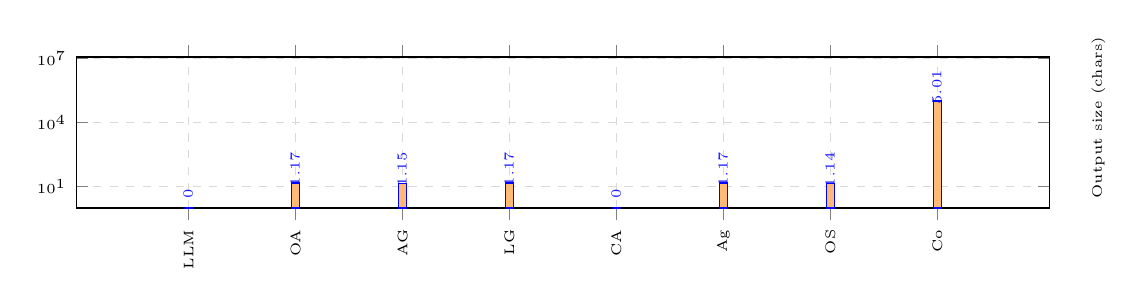
\begin{tikzpicture}
\begin{semilogyaxis}[
    width=1.15\linewidth,
    height=3.5cm,
    ymode=log,
    log basis y=10,
    ymin=1,
    ymax=11799100.564,
    % symbolic x coords={Direct LLM,OpenAgents,AutoGen,LangGraph,CrewAI,Agno,OpenAISDK,Concordia},
    symbolic x coords={ LLM,OA,AG,LG,CA,Ag,OS,Co},
    xtick=data,
    grid=major,
    xticklabel style={rotate=90, anchor=east, font=\tiny},
    ylabel={Output size (chars)},
    ylabel style={at={(axis description cs:1.05,0.)}, anchor=west},
    tick label style={font=\tiny},
    ymajorgrids=true,
    grid style=dashed,
    ylabel style={font=\tiny},
    xlabel style={font=\tiny},
    ybar,
    bar width=3pt,
    enlarge x limits=0.15,
    ymajorgrids=true,
    grid style={dashed,gray!30},
    nodes near coords,
    nodes near coords style={
        font=\tiny,
        yshift=5pt,
        xshift=5pt,
        anchor=south,
        rotate=90
    },
    every axis plot/.append style={fill opacity=0.9}
]
% \addplot+[fill=orange!60] coordinates {(Direct LLM,1.000) (OpenAgents,14.900) (AutoGen,14.220) (LangGraph,14.900) (CrewAI,1.000) (Agno,14.800) (OpenAISDK,13.880) (Concordia,102601.360)};
\addplot+[fill=orange!60] coordinates {
    (LLM,1.000) (OA,14.900) (AG,14.220) (LG,14.900)
    (CA,1.000) (Ag,14.800) (OS,13.880) (Co,102601.360)
};

\end{semilogyaxis}
\end{tikzpicture}
\vspace{-3mm}
\caption{Mean output}
\end{subfigure}
% ---------------- Output Summary ----------------
\hspace{-4mm} 
\begin{subfigure}{0.57\linewidth}
%\centering
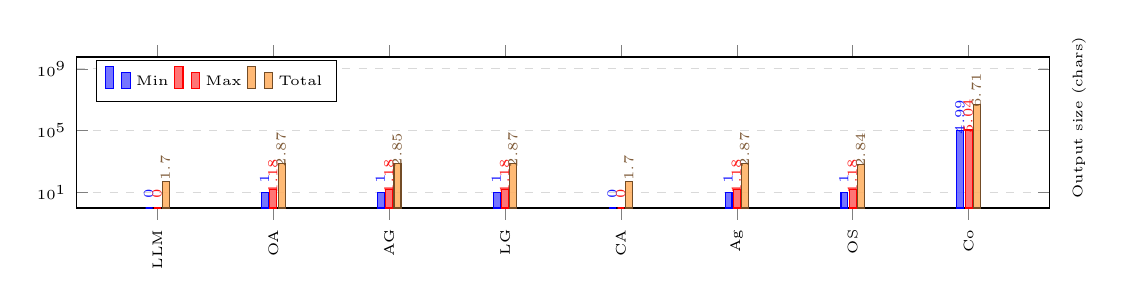
\begin{tikzpicture}
\begin{axis}[
    width=1.15\linewidth,
    height=3.5cm,
    ymode=log,
    log basis y=10,
    ymin=1,
    ymax=5899578000.200,
    % symbolic x coords={Direct LLM,OpenAgents,AutoGen,LangGraph,CrewAI,Agno,OpenAISDK,Concordia},
    symbolic x coords={ LLM,OA,AG,LG,CA,Ag,OS,Co},
    xtick=data,
    xticklabel style={rotate=90, anchor=east, font=\tiny},
    ylabel={Output size (chars)},
    ylabel style={at={(axis description cs:1.03,0.)}, anchor=west},
    legend style={
    at={(0.02,0.98)},
    anchor=north west,
    font=\tiny,
    legend columns=-1
    },
    tick label style={font=\tiny},
    ylabel style={font=\tiny},
    xlabel style={font=\tiny},
    ybar,
    bar width=2.5pt,
    enlarge x limits=0.1,
    ymajorgrids=true,
    grid style={dashed,gray!30},
    nodes near coords,
    nodes near coords style={
        font=\tiny,
        yshift=5pt,
        xshift=5pt,
        anchor=south,
        rotate=90
    },
    every axis plot/.append style={fill opacity=0.9}
]
% \addplot+[fill=blue!60] coordinates {(Direct LLM,1.000) (OpenAgents,10.000) (AutoGen,10.000) (LangGraph,10.000) (CrewAI,1.000) (Agno,10.000) (OpenAISDK,10.000) (Concordia,97448.000)};
% \addplot+[fill=red!60] coordinates {(Direct LLM,1.000) (OpenAgents,15.000) (AutoGen,15.000) (LangGraph,15.000) (CrewAI,1.000) (Agno,15.000) (OpenAISDK,15.000) (Concordia,110886.000)};
% \addplot+[fill=orange!60] coordinates {(Direct LLM,50.000) (OpenAgents,745.000) (AutoGen,711.000) (LangGraph,745.000) (CrewAI,50.000) (Agno,740.000) (OpenAISDK,694.000) (Concordia,5130068.000)};
\addplot+[fill=blue!60, bar shift=-3pt] coordinates {
    (LLM,1.000) (OA,10.000) (AG,10.000) (LG,10.000)
    (CA,1.000) (Ag,10.000) (OS,10.000) (Co,97448.000)
};

\addplot+[fill=red!60, bar shift=-0pt] coordinates {
    (LLM,1.000) (OA,15.000) (AG,15.000) (LG,15.000)
    (CA,1.000) (Ag,15.000) (OS,15.000) (Co,110886.000)
};

\addplot+[fill=orange!60, bar shift=3pt] coordinates {
    (LLM,50.000) (OA,745.000) (AG,711.000) (LG,745.000)
    (CA,50.000) (Ag,740.000) (OS,694.000) (Co,5130068.000)
};

\legend{Min, Max, Total}
\end{axis}
\end{tikzpicture}
\vspace{-7mm}
\caption{Output summary}
\end{subfigure}
\hfill
\vspace{0mm}
\noindent\fbox{%
  \parbox{0.85\linewidth}{\scriptsize
  \textbf{Abbreviations:}
  LLM=Direct LLM;
  OA=OpenAgents;
  AG=AutoGen;
  LG=LangGraph; \\
  CA=CrewAI;
  Ag=Agno;
  OS=OpenAI SDK;
  Co=Concordia.
  }
}
\vspace{-4mm}
\caption{
Framework overhead on a trivial task (“What is 2+2?”) over 50 trials.
Frameworks are ordered by p50 latency.
}
\vspace{-4mm}
\label{fig:framework-overhead}
\end{figure}





% Figure~\ref{fig:framework-overhead} summarizes the framework overhead results across all evaluated systems, with Figure~\ref{fig:framework-overhead}(a) reporting median (p50) and tail (p95) latency and Figure~\ref{fig:framework-overhead}(b) reporting throughput under concurrent load. Direct LLM calls provide the lower bound on both metrics and serve as a reference point for all orchestration frameworks. Among lightweight orchestration approaches, AutoGen and OpenAgents achieve latency and throughput comparable to, and in several cases better than, the graph-based LangGraph runtime, indicating that role-based abstractions do not inherently imply higher overhead when execution remains shallow. LangGraph introduces only modest additional cost due to graph scheduling and state propagation, while other role-based frameworks such as CrewAI, Agno, and the OpenAI Agents SDK incur progressively higher overhead as agent initialization, role conditioning, prompt templating, and task execution logic are layered on. Across all non-generative frameworks, throughput trends closely mirror latency behavior, showing that per-request orchestration overhead directly constrains scalability under parallel workloads. In contrast, Concordia, which follows a generative-agent-based modeling (GABM) paradigm, operates in a qualitatively different regime: both median and tail latencies increase by more than an order of magnitude, reaching tens of seconds, while throughput collapses to nearly zero. This sharp separation reflects the fundamental cost of Concordia’s simulation-centric execution model, which performs full environment stepping, narrative observation generation, and Game Master resolution even for trivial queries rather than a lightweight request–response interaction. Additional details on Concordia’s execution trace—and why its simulation pipeline prevents direct numeric outputs—are provided in Appendix~\ref{sec:concordia_appendix}.




% Figure~\ref{fig:framework-overhead}(c) reports the mean output size per request on a logarithmic scale, while Figure~\ref{fig:framework-overhead}(d) summarizes the minimum, maximum, and total output sizes across all trials. Direct LLM calls produce the minimal expected output, serving as a lower-bound baseline in both mean and total generation. Graph-based orchestration (LangGraph) and lightweight role-based frameworks such as AutoGen and OpenAgents generate slightly longer outputs, typically short natural-language responses or brief explanations, resulting in output sizes clustered around $10^1$ to $10^2$ characters; notably, AutoGen and OpenAgents remain comparable to, and in some cases more concise than, LangGraph, indicating that role-based abstractions do not inherently inflate generation length when execution remains shallow. More feature-rich role-based frameworks, including CrewAI, Agno, and the OpenAI Agents SDK, exhibit modestly larger variance but still maintain tightly bounded minimum and maximum outputs, leading to predictable total output sizes that scale linearly with the number of trials. In contrast, Concordia deviates by several orders of magnitude: its mean output size exceeds $10^4$ characters, its minimum per-run output surpasses the maximum output of all other frameworks, and the cumulative output across 50 trials reaches millions of characters. This behavior is not a measurement artifact but a direct consequence of Concordia’s simulation-centric architecture, which emits full narrative transcripts, structured action specifications, and complete environment state transitions rather than a concise task answer. Taken together with the latency and throughput results, these findings highlight a clear trade-off between abstraction and efficiency: lightweight graph-based and role-based frameworks introduce manageable overhead suitable for interactive and high-throughput settings, whereas Concordia occupies a fundamentally different design regime in which substantially higher output volume and execution cost are deliberate architectural choices, as detailed further in Appendix~\ref{sec:concordia_appendix}.





% \vspace{-2mm}
% \subsubsection{Framework Overhead}
% \label{sec:framework-overhead}

% We first quantify the baseline overhead imposed by multi-agent frameworks relative to a direct Large Language Model (LLM) invocation. This experiment isolates orchestration cost from advanced capabilities such as tool use, memory, planning, or inter-agent coordination, and establishes a lower-bound reference for interpreting all subsequent results. All frameworks are evaluated under identical conditions using a trivial query (\emph{``What is 2+2?''}), the same model (\emph{gpt-4o-mini}), and a unified execution pipeline. Each framework is configured in its minimal viable setting, disabling optional features to focus exclusively on orchestration behavior. The comparison includes a raw \emph{Direct LLM} call as a baseline; lightweight graph-based (\emph{LangGraph}) and role-based frameworks (\emph{OpenAgents}, \emph{AutoGen}, \emph{CrewAI}, \emph{Agno}, and the \emph{OpenAI SDK}); and the generative-agent-based modeling (GABM) system \emph{Concordia}. Each configuration is executed for 50 trials with fixed concurrency, and we report latency, throughput, and output size.


% Figure~\ref{fig:framework-overhead}(a,b) reports latency and throughput under concurrent load. Direct LLM calls provide the lower bound on both metrics. Among lightweight frameworks, AutoGen and OpenAgents achieve latency and throughput comparable to LangGraph, indicating that role-based abstractions do not inherently increase overhead when execution remains shallow. LangGraph incurs modest additional cost due to graph scheduling and state propagation, while CrewAI, Agno, and the OpenAI SDK exhibit progressively higher overhead as role conditioning, prompt templating, and task logic accumulate. Throughput closely mirrors latency across all non-GABM frameworks, showing that per-request orchestration cost directly constrains scalability. In contrast, Concordia operates in a different execution model. Median and tail latency increase by more than an order of magnitude, while throughput collapses, reflecting its simulation-centric model rather than request–response interaction.\footnote{\vspace{-3mm} More details about Concordia behavior are provided in the \uline{\textcolor{blue}{\href{https://github.com/CoDS-GCS/MAFBench/blob/main/supplementary_materials/APPENDICIES.pdf}{supplementary materials}}}.}
% % More details about Concordia behavior are provided in Appendix~\ref{sec:concordia_appendix}.




% Figure~\ref{fig:framework-overhead}(c,d) reports output size statistics. Direct LLM calls produce minimal output, while LangGraph, AutoGen, and OpenAgents generate slightly longer but bounded responses. More feature-rich role-based frameworks show higher variance but remain predictable. Concordia deviates sharply, producing outputs several orders of magnitude larger due to narrative transcripts, environment state emissions, and Game Master mediation. Taken together, these results reveal a clear separation between workflow-oriented frameworks with manageable overhead and simulation-centric architectures with higher cost. This separation is independent of task difficulty and reflects an intrinsic execution model imposed by framework design.



% 


\captionsetup[subfigure]{font=scriptsize}
\begin{figure}[t]
%\centering
\begin{subfigure}{0.57\linewidth}
% %\centering
\begin{tikzpicture}
\begin{groupplot}[
    group style={
        group size=1 by 2,
        vertical sep=0.4cm, % Gap between the two plots
        x descriptions at=edge bottom, % Only show x labels on bottom plot
    },
    width=1.25\linewidth,
    symbolic x coords={LLM,OA,AG,LG,CA,Ag,OS,Co},
    xtick=data,
    ybar,
    % bar width=3pt,
    /pgf/bar width=3pt,
    enlarge x limits=0.15,
    ymajorgrids=true,
    grid style={dashed,gray!30},
    tick label style={font=\tiny},
    ylabel style={font=\tiny},
    xlabel style={font=\tiny},
    every axis plot/.append style={fill opacity=0.9},
    nodes near coords,
    nodes near coords style={
        font=\tiny, yshift=7pt, xshift=5pt, anchor=south, rotate=90
    }
]

% --- TOP PLOT (Outlier Range) ---
\nextgroupplot[
    height=2.5cm,
    ymin=44, ymax=70, % Range for Concordia
    ytick={40, 50, 60},
    axis x line*=top
, % Hide the x-axis for the top part
    legend style={
        at={(0.02,0.98)},
        anchor=north west,
        font=\tiny,
        legend columns=-1
    },
    ylabel={Latency (s)},
    ylabel style={at={(axis description cs:1.03, -1.2)}, anchor=west}, % Centered label
]
\addplot+[fill=blue!60] coordinates {
    (LLM,0.379) (OA,0.495) (AG,0.496) (LG,0.524)
    (CA,0.611) (Ag,0.860) (OS,1.170) (Co,44.473)
};
\addplot+[fill=green!60] coordinates {
    (LLM,0.730) (OA,0.840) (AG,0.787) (LG,1.093)
    (CA,0.801) (Ag,1.183) (OS,2.036) (Co,53.420)
};
\legend{p50, p95}

% --- BOTTOM PLOT (Main Data Range) ---
\nextgroupplot[
    height=2.3cm,
    ymin=0, ymax=3, % Range for all other agents
    ytick={0, 1, 2, 3},
    axis x line*=bottom,
    xticklabel style={rotate=90, anchor=east, font=\tiny},
    % axis y discontinuity=parallel, % Adds the visual "break" symbol
]
\addplot+[fill=blue!60] coordinates {
    (LLM,0.379) (OA,0.495) (AG,0.496) (LG,0.524)
    (CA,0.611) (Ag,0.860) (OS,1.170) (Co,44.473)
};
\addplot+[fill=green!60] coordinates {
    (LLM,0.730) (OA,0.840) (AG,0.787) (LG,1.093)
    (CA,0.801) (Ag,1.183) (OS,2.036) (Co,53.420)
};

\end{groupplot}
\end{tikzpicture}
\vspace{-7mm}
\caption{Latency}
\end{subfigure}
% \hspace{1mm}
% \hfill
% ---------------- Throughput ----------------
\begin{subfigure}{0.42\linewidth}
%\centering
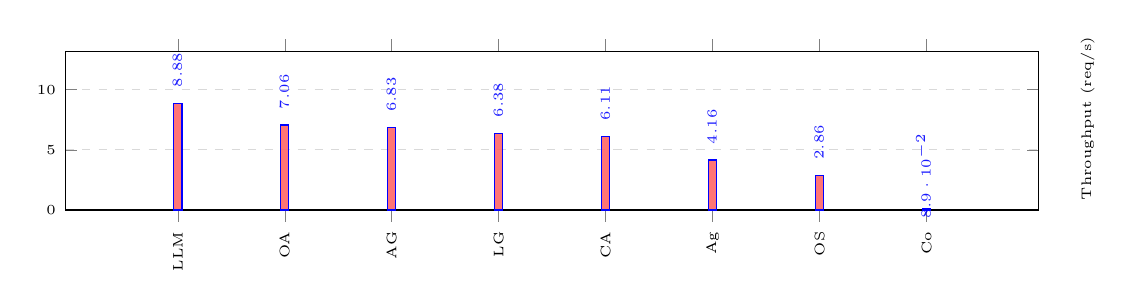
\begin{tikzpicture}
\begin{axis}[
    width=1.15\linewidth,
    height=3.6cm,
    ymin=0,
    ymax=13.206,
    % symbolic x coords={Direct LLM,OpenAgents,AutoGen,LangGraph,CrewAI,Agno,OpenAISDK,Concordia},
    symbolic x coords={ LLM,OA,AG,LG,CA,Ag,OS,Co},
    xtick=data,
    xticklabel style={rotate=90, anchor=east, font=\tiny},
    ylabel={Throughput (req/s)},
    ylabel style={at={(axis description cs:1.05,0.)}, anchor=west},
    tick label style={font=\tiny},
    ylabel style={font=\tiny},
    xlabel style={font=\tiny},
    ybar,
    bar width=3pt,
    enlarge x limits=0.15,
    ymajorgrids=true,
    grid style={dashed,gray!30},
    nodes near coords,
    nodes near coords style={
        font=\tiny,
        yshift=12pt,
        xshift=5pt,
        anchor=south,
        rotate=90
    },
    every axis plot/.append style={fill opacity=0.9},
]
% \addplot+[fill=red!60] coordinates {(Direct LLM,8.875) (OpenAgents,7.062) (AutoGen,6.827) (LangGraph,6.377) (CrewAI,6.113) (Agno,4.158) (OpenAISDK,2.860) (Concordia,0.089)};
\addplot+[fill=red!60] coordinates {(LLM,8.875) (OA,7.062) (AG,6.827) (LG,6.377) (CA,6.113) (Ag,4.158) (OS,2.860) (Co,0.089)};
\end{axis}
\end{tikzpicture}
\vspace{-3mm}
\caption{Throughput}
\end{subfigure}


\hspace{-2mm}
% ---------------- Mean Output ---------------- 
\begin{subfigure}{0.42\linewidth}
%\centering
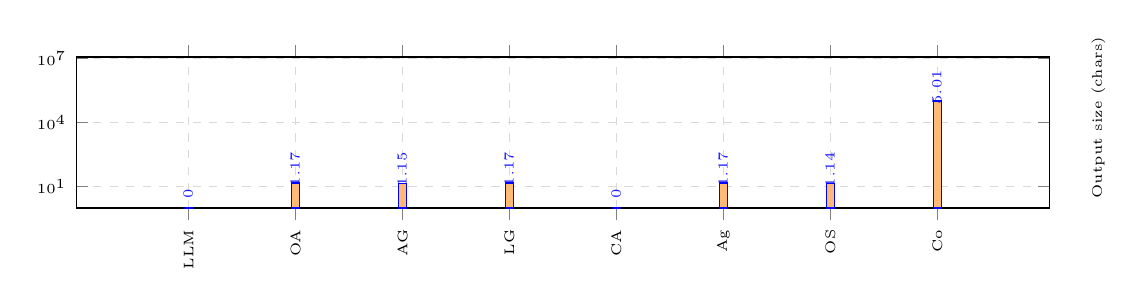
\begin{tikzpicture}
\begin{semilogyaxis}[
    width=1.15\linewidth,
    height=3.5cm,
    ymode=log,
    log basis y=10,
    ymin=1,
    ymax=11799100.564,
    % symbolic x coords={Direct LLM,OpenAgents,AutoGen,LangGraph,CrewAI,Agno,OpenAISDK,Concordia},
    symbolic x coords={ LLM,OA,AG,LG,CA,Ag,OS,Co},
    xtick=data,
    grid=major,
    xticklabel style={rotate=90, anchor=east, font=\tiny},
    ylabel={Output size (chars)},
    ylabel style={at={(axis description cs:1.05,0.)}, anchor=west},
    tick label style={font=\tiny},
    ymajorgrids=true,
    grid style=dashed,
    ylabel style={font=\tiny},
    xlabel style={font=\tiny},
    ybar,
    bar width=3pt,
    enlarge x limits=0.15,
    ymajorgrids=true,
    grid style={dashed,gray!30},
    nodes near coords,
    nodes near coords style={
        font=\tiny,
        yshift=5pt,
        xshift=5pt,
        anchor=south,
        rotate=90
    },
    every axis plot/.append style={fill opacity=0.9}
]
% \addplot+[fill=orange!60] coordinates {(Direct LLM,1.000) (OpenAgents,14.900) (AutoGen,14.220) (LangGraph,14.900) (CrewAI,1.000) (Agno,14.800) (OpenAISDK,13.880) (Concordia,102601.360)};
\addplot+[fill=orange!60] coordinates {
    (LLM,1.000) (OA,14.900) (AG,14.220) (LG,14.900)
    (CA,1.000) (Ag,14.800) (OS,13.880) (Co,102601.360)
};

\end{semilogyaxis}
\end{tikzpicture}
\vspace{-3mm}
\caption{Mean output}
\end{subfigure}
% ---------------- Output Summary ----------------
\hspace{-4mm} 
\begin{subfigure}{0.57\linewidth}
%\centering
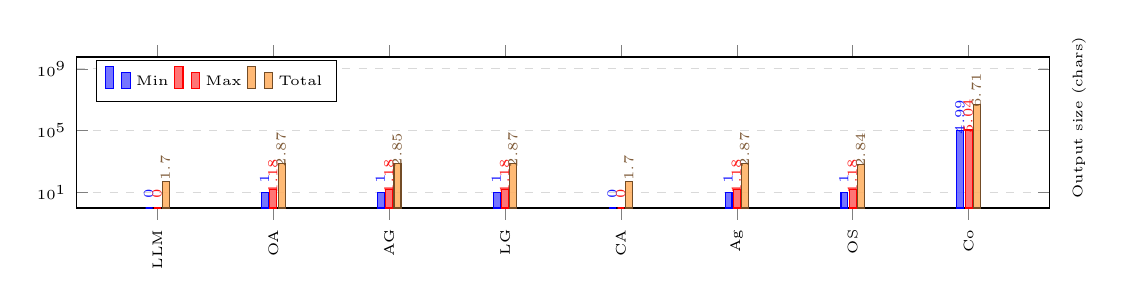
\begin{tikzpicture}
\begin{axis}[
    width=1.15\linewidth,
    height=3.5cm,
    ymode=log,
    log basis y=10,
    ymin=1,
    ymax=5899578000.200,
    % symbolic x coords={Direct LLM,OpenAgents,AutoGen,LangGraph,CrewAI,Agno,OpenAISDK,Concordia},
    symbolic x coords={ LLM,OA,AG,LG,CA,Ag,OS,Co},
    xtick=data,
    xticklabel style={rotate=90, anchor=east, font=\tiny},
    ylabel={Output size (chars)},
    ylabel style={at={(axis description cs:1.03,0.)}, anchor=west},
    legend style={
    at={(0.02,0.98)},
    anchor=north west,
    font=\tiny,
    legend columns=-1
    },
    tick label style={font=\tiny},
    ylabel style={font=\tiny},
    xlabel style={font=\tiny},
    ybar,
    bar width=2.5pt,
    enlarge x limits=0.1,
    ymajorgrids=true,
    grid style={dashed,gray!30},
    nodes near coords,
    nodes near coords style={
        font=\tiny,
        yshift=5pt,
        xshift=5pt,
        anchor=south,
        rotate=90
    },
    every axis plot/.append style={fill opacity=0.9}
]
% \addplot+[fill=blue!60] coordinates {(Direct LLM,1.000) (OpenAgents,10.000) (AutoGen,10.000) (LangGraph,10.000) (CrewAI,1.000) (Agno,10.000) (OpenAISDK,10.000) (Concordia,97448.000)};
% \addplot+[fill=red!60] coordinates {(Direct LLM,1.000) (OpenAgents,15.000) (AutoGen,15.000) (LangGraph,15.000) (CrewAI,1.000) (Agno,15.000) (OpenAISDK,15.000) (Concordia,110886.000)};
% \addplot+[fill=orange!60] coordinates {(Direct LLM,50.000) (OpenAgents,745.000) (AutoGen,711.000) (LangGraph,745.000) (CrewAI,50.000) (Agno,740.000) (OpenAISDK,694.000) (Concordia,5130068.000)};
\addplot+[fill=blue!60, bar shift=-3pt] coordinates {
    (LLM,1.000) (OA,10.000) (AG,10.000) (LG,10.000)
    (CA,1.000) (Ag,10.000) (OS,10.000) (Co,97448.000)
};

\addplot+[fill=red!60, bar shift=-0pt] coordinates {
    (LLM,1.000) (OA,15.000) (AG,15.000) (LG,15.000)
    (CA,1.000) (Ag,15.000) (OS,15.000) (Co,110886.000)
};

\addplot+[fill=orange!60, bar shift=3pt] coordinates {
    (LLM,50.000) (OA,745.000) (AG,711.000) (LG,745.000)
    (CA,50.000) (Ag,740.000) (OS,694.000) (Co,5130068.000)
};

\legend{Min, Max, Total}
\end{axis}
\end{tikzpicture}
\vspace{-7mm}
\caption{Output summary}
\end{subfigure}
\hfill
\vspace{0mm}
\noindent\fbox{%
  \parbox{0.85\linewidth}{\scriptsize
  \textbf{Abbreviations:}
  LLM=Direct LLM;
  OA=OpenAgents;
  AG=AutoGen;
  LG=LangGraph; \\
  CA=CrewAI;
  Ag=Agno;
  OS=OpenAI SDK;
  Co=Concordia.
  }
}
\vspace{-4mm}
\caption{
Framework overhead on a trivial task (“What is 2+2?”) over 50 trials.
Frameworks are ordered by p50 latency.
}
\vspace{-4mm}
\label{fig:framework-overhead}
\end{figure}








\vspace{-2mm}
\subsubsection{Framework Overhead}
\label{sec:framework-overhead}

We evaluate how orchestration architecture affects baseline execution cost in multi-agent frameworks, independent of memory, planning, tool use, and coordination. Using a unified execution pipeline, we fix the LLM (\emph{gpt-4o-mini}), the query (\emph{``What is 2+2?''}), prompts, and concurrency, and vary only the framework orchestration layer under minimal viable configurations. The comparison includes a raw \emph{Direct LLM} baseline; graph- and role-based frameworks \emph{LangGraph}~\cite{langgraph2025}, \emph{OpenAgents}~\cite{OpenAgents}, \emph{AutoGen}~\cite{wu2024autogen}, \emph{CrewAI}~\cite{crewai2025}, \emph{Agno}~\cite{agno2025}, and the \emph{OpenAI SDK}~\cite{openaiagents2025}; and the GABM framework \emph{Concordia}~\cite{vezhnevets2023generative}. We run 50 trials and report median (p50) and tail (p95) latency, throughput, and output size. 

Figure~\ref{fig:framework-overhead}(a,b) shows that Direct LLM calls achieve the lowest latency and highest throughput. AutoGen and OpenAgents closely match LangGraph, indicating minimal overhead for shallow role-based abstractions. LangGraph incurs modest additional cost from graph scheduling and state propagation, while CrewAI, Agno, and the OpenAI SDK exhibit progressively higher latency as orchestration logic increases, with throughput mirroring latency across graph- and role-based frameworks. In contrast, Concordia shows more than an order-of-magnitude increase in median and tail latency and a sharp drop in throughput, reflecting its GABM execution semantics. Output sizes in Figure~\ref{fig:framework-overhead}(c,d), shown on a logarithmic scale, remain bounded for graph- and role-based frameworks but grow by several orders of magnitude for Concordia due to narrative transcripts and environment-mediated state updates. Additional Concordia analysis appears in Appendix~\ref{sec:concordia_appendix}. 
%
Overall, these results show that orchestration architecture alone governs baseline scalability. Graph- and role-based designs introduce modest but compounding overhead over direct LLM execution, whereas GABM execution incurs orders-of-magnitude higher runtime and output even for trivial tasks, driven by execution semantics rather than task complexity.











